
}
\chapter[Digging up QTL: Evaluating the efficiency of marker-assisted selection in hybrid potato]{Digging up QTL: Evaluating the efficiency of marker-assisted selection in hybrid potato}
\chaptermark{Evaluating the efficiency of marker-assisted selection in hybrid potato}
\label{cha:chapter4}
\vspace*{\fill}

\newpage

\section*{Abstract}

Hybrid potato is a novel crop strategy which develops cultivars with improved F1 
hybrids created from inbred diploid potato lines. As with other crops,
the hybrid breeding system allows for greater flexibility and
potentially greater speed in contrast to traditional tetraploid potato
breeding. An important aspect of how a hybrid breeding program should be
structured is resource and technology allocation for optimum selection efficiency.
The authors of this paper examined this question with respect to marker
and selection technologies examining the relative efficiency of
marker-assisted selection (\texttt{MA}) relative to a traditional
genome-wide selection (\texttt{GW}) for F4 candidate selection. For the MA scenario, we were
able to identify 35 QTL for all tuber phenotypes that accounted for a large portion of the genetic variation in multiple yield components. The \texttt{GW} strategy
had the highest prediction accuracy with relative selection efficiency's
consistent with this for all traits. However, when examining the
relative efficiency with respect to cost of genotyping strategy, the
\texttt{MA} scenario was more efficient for all traits studied here. Our
findings suggest that marker-assisted selection could be an attractive
method for quantitative trait selection in commercial hybrid potato
programs.

\newpage

\section{Introduction}

Potato (\emph{Solanum tuberosum} L.) is the newest field crop
undergoing conversion to a hybrid breeding system
\autocite{DeVries2023,Jansky2016}. Following the success of other crops
like sugar beet \autocite{McGrath2018} and sunflower
\autocite{Dimitrijevic2018}, both private and public ventures are
endeavouring to convert this clonal tetraploid crop into a diploid
chasing the same benefits that were originally observed in maize
\autocite{Duvick1997}. This conversion in potato is actually composed of
two distinct and yet inter-related activities: (1) ploidy reduction from
a tetraploid to diploid, and (2) the shift from outcrossing populations
to structured inbred populations shaped around F1 hybrid performance.
The benefits of the former primarily lie in the ease and speed of
positive gene fixation in a disomic inheritance model over tetrasomic
inheritance \autocite{Hougas1958} with the latter comprising both
technical (trait fixation in inbreds, exploitation of heterotic vigour)
and commercial (intellectual property protection, consistent product
quality and uniformity) related advantages \autocite{Wright1980}.
Despite the allure of these propositions, it is only within the past
decade that commercialization efforts of hybrid potato programs have
come to pass due in part to overcoming genetic barriers like severe
inbreeding depression, fertility anomalies, and ploidy barriers for
secondary and tertiary gene pools
\autocite{Zhang2019,Endelman2016,Zhang2021}.

It is well understood that while hybrid breeding systems bring many
potential benefits to crop improvement strategies, this is not without
significant cost. Hybrid breeding is known to suffer from longer
breeding cycles in contrast to line breeding and necessitates specific
populations for heterotic pool development
\autocite{Labroo2021,Longin2013}. A large aspect of that complexity lies
in that the target for improvement is F1 performance and not inbred
family \emph{per se} yields due to poor correlations between the two. In
the pre-genomics era, testcross evaluation was the crux of line
advancement and population enrichment as it permitted the estimation of
general and specific combining abilities \autocite{Carangal1971}. It was
not until the advent of molecular technologies that it became possible
to develop inexpensive proxies in the place of field evaluation, first
in the form of molecular markers for marker-assisted selection (MAS) not
long followed by genome-wide regression using hundreds to thousands of
markers for genomic selection (GS) \autocite{Lande1990,Meuwissen2001}.
These methods alone have been responsible for incredible gains for
quantitative trait improvement in field and vegetable crops alike over
the past 30 years.

While genome-wide selection is a powerful tool in quantitative trait
improvement, it is not necessarily the most \emph{efficient}.
Genome-wide selection has been shown to work very well in both
tetraploid and diploid potato populations
\autocite{Adams2023,Wilson2021}, but the cost associated with training
set development, dense molecular marker panels, and computational
capacity make it a resource-intensive process. An interesting
alternative would be identifying quantitative traits which could be
selected solely on the basis of QTL information. The literature is ripe
with examples of large-effect QTL responsible for controlling traits
such as tuber shape \autocite{Eck2022}, starch content
\autocite{Li2019a}, maturity \autocite{Li2018,Massa2015} and even volume
and weight of tubers \autocite{Korontzis2020,Clot2024}. Making these
identified QTL the basis of selection in a MAS program could be a simple
and and cost-effective method for improving quantitative trait targets in
potato. However, while the success of MAS is well understood in other
crops and simulation \autocite{Podlich2004, VanBerloo2008}, its utility in hybrid
potato is currently unknown. We examine the following scenarios: a
marker-assisted breeding scenario which conducts selection based on
identified QTL in the hybrid (\texttt{MA}), a genome-wide selection
method (\texttt{GW}), and lastly a method which bases selection on 1
random SNP per chromosome (\texttt{PC}). These three strategies were
assessed on their prediction accuracy for the tuber phenotype as well as
on the relative efficiency with respect to genome-wide selection. With
these results, we hope to identify if marker-assisted selection is a
useful selection method in practice for complex traits in potato.
\section{Material and methods}

\subsection{Hybrid Phenotypic Data}\label{hybrid-phenotypic-data}

This study used a population of 785 genotyped F1 hybrids which had
undergone field evaluation between 2019 and 2020. As described in
\autocite{Adams2023}, this dataset comprises four field trials in two
trial locations (Heelsum and Est, Netherlands). Best linear unbiased
predictions (BLUPs) for hybrids were computed using the following model:

\begin{equation}\protect\hypertarget{eq-blup-model}{}{ y_{bfht} = \beta_f +\gamma_{fb} + a_{ht} + \varepsilon_{bfht} }\label{eq-blup-model}\end{equation}

where \(y\) is some component of yield for hybrid \(h\) within block
\(b\) in trial location \(t\) and specific field trial \(f\). \(y\) is
modeled on a fixed trial (\(\beta_f\)) and block within-trial
(\(\gamma_{fb}\)) effects, a random hybrid by trial (\(a_{ht}\)), and an
independent and identically distributed (IID) residual term
(\(\varepsilon_{bfht}\)). The hybrid by trial effect was modeled as
Gaussian with an unstructured variance structure:

\[a \sim \mathrm{N} \left (\mathbf{0},  \Sigma_a \right )  ~~~~~~~~~~~~~  \Sigma_a =\begin{bmatrix} \sigma^2_{\mathrm{G(Est)}} &  \sigma_{\mathrm{G(Est),G(Hee)}}\\ \sigma_{\mathrm{G(Hee),G(Est)}} & \sigma^2_{\mathrm{G(Hee)}}\end{bmatrix}\]

This model structure was chosen over simpler multi-environment models
due to large observed differences in genetic variances during
exploratory analysis. Such large discrepancies in variance were not
observed for the residual term across trials so this retained its IID
variance structure. Several variates were analyzed including including
total tuber yield (TY; \(\mathrm Mg \cdot \mathrm{Ha^{-1}}\)), tuber dry
matter content (DM; per cent), and average tuber volume (TV; \(cm^3\)).

\hypertarget{marker-processing}{%
\subsection{Marker processing}\label{marker-processing}}

Using the same dataset described in \autocite{Adams2023}, marker data
was collected on the 416 parental lines used in the creation of the
evaluated hybrids. These lines were genotyped with a targeted
genotyping-by-sequencing (GBS) technology marketed as SeqSNP and
developed by LGC \autocite{LGC2019}. For this analysis, single
nucleotide polymorphism's (SNPs) were extracted and filtered from the
probeset and filtered based upon SNP missingness, minor allele
frequency, and SNP density. These filter criteria left 1,040 remaining
SNP's which were used to infer F1 hybrid genotypes for QTL mapping and
genome-wide prediction.

\hypertarget{qtl-scanning-and-incorporation}{%
\subsection{QTL Scanning and
Incorporation}\label{qtl-scanning-and-incorporation}}

QTL scans were conducted on all phenotypes using the hybrid BLUPs
averaged over location and standard errors produced from ASReml-R's
\texttt{predict()} interface along with SNP data. This was done using a
forward-selection approach. The null model has the following form:

\begin{equation}\protect\hypertarget{eq-null-model}{}{ \hat{\mathbf{y}} = \mathbf{1}\mu + \mathrm{X_Q}\beta_{Q} + \mathrm{Z_g}u + e }\label{eq-null-model}\end{equation}

where \(\hat{\mathbf{y}}\) is the vector of hybrid predictions, \(\mu\)
is the global mean, \(\beta_Q\) is a vector of QTL fixed effects, \(u\)
is a vector of random background genetic effects
(\(u \sim \mathrm{N}(0, \sigma^2_g)\)), and \(e\) is a vector of
residuals whose variance is structured from the first-stage model
standard errors
(\(e\sim \mathrm{N}(0, \mathrm{R = Diag(\hat{se^2_1}, \hat{se^2_2}, \ldots, \hat{se^2_n})})\)).
During the first QTL scan, \(X_Q\), the design matrix which contains SNP
dosage of previously identified QTL, and \(\beta_Q\) will be empty. The
design matrix for the background genetic effects, \(\mathrm Z_g\), is a
diagonal matrix.

This model is tested against a scanning model:

\begin{equation}\protect\hypertarget{eq-scan-model}{}{ \hat{\mathbf{y}} = \mathbf{1}\mu + \mathrm{X_Q}\beta_{Q} + \mathrm{Z_g}u + \mathrm{Z_{snp}}v + e }\label{eq-scan-model}\end{equation}

which differs only in the addition of one random term, \(v\), the SNP
effect (\(v \sim \mathrm{N(0,}\sigma^2_{qtl}\)) being tested at any
given scan. The forward-selection procedure consisted of: (1) fitting
the null model in (Equation~\ref{eq-null-model}), (2) fitting the
scanning model (Equation~\ref{eq-scan-model}), (3) conducting a
likelihood ratio test to assess the significance of \(v\), (4) repeating
steps 2-3 for all remaining SNPs, (5) selecting the SNP with the
smallest p-value and placing it in \(\mathrm{X}\) if it was smaller than
the cutoff (defined by a Bonferroni threshold) and then repeating. If
there were no remaining SNPs with sufficient evidence of putative QTL,
the scan was concluded. A Wald test was then conducted on the final
model to confirm the significance of all QTL in \(\mathrm{X_Q}\); the
effect size of all QTLs were extracted from this model
(Figure~\ref{fig-snp-size}). While some QTLs clustered within close proximity to one another, all QTL distances were above 1 Mb and thus considered independent of one another. Lastly, each QTL was fit in a single QTL
model
(\(\hat{\mathbf{y}} = \mathbf{1}\mu + \mathrm{Z_g}u + \mathrm{Z_{snp}}v + e\))
to estimate the proportion of QTL variance (Figure~\ref{fig-gen-size}).

The number of QTL taken up in each model was recorded
(Table~\ref{tbl-summary}) along with their significance
(i.e.~\(- \mathrm{log}_{10}(p)\)) during initial model scanning
(Figure~\ref{fig-lod-score}). All QTL modeling and phenotypic analyses
were done using ASReml-R 4.2 \autocite{Butler2017}.

\subsection{Genomic Prediction Models}\label{genomic-prediction-models}

Because one of the major research questions was related to testing the
utility of a multi-QTL model in a marker-assisted selection program, we constructed
multiple prediction models associated with distinct modeling scenarios
(See Table~\ref{tbl-scenarios}). The first was a marker-assisted
selection model (\texttt{MA}) which bases prediction upon the previously
identified QTL (Table~\ref{tbl-summary}). All QTL which were found to be
jointly significant were incorporated into a traditional linear
regression model to predict a candidate's value among our selected
quantitative traits. This model was:

\begin{equation}\protect\hypertarget{eq-mas-model}{}{ \hat{\mathbf{y}} = \mathbf{1}\mu + \mathrm{X}_Q\beta_Q + \varepsilon }\label{eq-mas-model}\end{equation}

where the hybrid BLUPs were modeled only on the global mean, and
estimated QTL effects (\(\beta_Q\)) in each hybrid. This scenario was
contrasted against a genome-wide based regression using 1000 SNPs
(\texttt{GW}) and a model which picks one random SNP per chromosome
(\texttt{PC}). The latter is meant to perform as a negative control to
evaluate the minimum performance threshold from a SNPs linkage within a
linkage group. Both of these models were trained using ridge
regression and could be expressed as:

\begin{equation}\protect\hypertarget{eq-rr-model}{}{ \hat{\mathbf{y}} =  \mathbf{1}\mu + \mathrm{W}u + \varepsilon }\label{eq-rr-model}\end{equation}

where the SNP dosages are contained in matrix, \(\mathrm{W}\), and all
marker effects in \(u\). To assess prediction performance, all models
were tested using 5-fold cross-validation. Cross-validation was
replicated 100 times for each trait for the \texttt{MA} model and
Pearson correlation coefficients were estimated for each fold and then
averaged over each replicate. For models which introduced marker
sampling variation (i.e., \texttt{GW} and \texttt{PC}), the replication
was stratified over marker sampling (\(n = 20\)) and fold partitioning
of hybrids (\(m = 50\)) for a total of 1000 replications. Similarly,
the predictive performance was assessed via the Pearson correlation
coefficient between the true and predicted hybrid performance and
averaged over each fold. The average Pearson correlation coefficient
were then compared across all models and traits (Figure~\ref{fig-pa}).
All prediction models were trained and tested used the
\texttt{mixed.solve()} function provided through the rrBLUP R library
\autocite{Endelman2011}.

\hypertarget{tbl-scenarios}{}
\begin{longtable}[]{@{}
  >{\raggedright\arraybackslash}p{(\columnwidth - 8\tabcolsep) * \real{0.0952}}
  >{\raggedright\arraybackslash}p{(\columnwidth - 8\tabcolsep) * \real{0.3333}}
  >{\raggedright\arraybackslash}p{(\columnwidth - 8\tabcolsep) * \real{0.1905}}
  >{\raggedright\arraybackslash}p{(\columnwidth - 8\tabcolsep) * \real{0.1905}}
  >{\raggedright\arraybackslash}p{(\columnwidth - 8\tabcolsep) * \real{0.1905}}@{}}
\caption{\label{tbl-scenarios}Breeding scenarios with descriptions of
model parameters and cost associated with each.}\tabularnewline
\toprule\noalign{}
\begin{minipage}[b]{\linewidth}\raggedright
Scenario code
\end{minipage} & \begin{minipage}[b]{\linewidth}\raggedright
Scenario
\end{minipage} & \begin{minipage}[b]{\linewidth}\raggedright
\(\hat{\beta}\)
\end{minipage} & \begin{minipage}[b]{\linewidth}\raggedright
\(\hat{u}\)
\end{minipage} & \begin{minipage}[b]{\linewidth}\raggedright
Cost
\end{minipage} \\
\midrule\noalign{}
\endfirsthead
\toprule\noalign{}
\begin{minipage}[b]{\linewidth}\raggedright
Scenario code
\end{minipage} & \begin{minipage}[b]{\linewidth}\raggedright
Scenario
\end{minipage} & \begin{minipage}[b]{\linewidth}\raggedright
X
\end{minipage} & \begin{minipage}[b]{\linewidth}\raggedright
W
\end{minipage} & \begin{minipage}[b]{\linewidth}\raggedright
Cost
\end{minipage} \\
\midrule\noalign{}
\endhead
\bottomrule\noalign{}
\endlastfoot
MA & Marker-assisted selection with identified QTLs & Identified QTL & &
\$0.15 per SNP per sample \\
GW & Genome-wide regression using mid-sized probe set & global mean &
1000 genome-wide SNP's & \$150.00 per sample \\
PC & Selection with one random SNP on each chromosome & global mean & 1
SNP per chromosome & \$1.80 per per sample \\
\end{longtable}

Putting the model performance in the context of a breeding program, we
examine \texttt{MA}, \texttt{PC}, and \texttt{GW} as alternative
modeling methods for predicting the genetic value of 1000 novel F4
candidates for creating superior F1 candidates. This is done on the basis of marker effect estimation at the F1 hybrid level which would make inbred selection based on that line's geonmically estimated breeding value. These schemas were evaluated
based on the relative efficiency for the \texttt{MA} and \texttt{PC}
scenarios relative to \texttt{GW} (Table~\ref{tbl-scenarios}). This is
the ratio of the predicted selection response (\(i\sigma_gr\)) of each
scenario over the genome-wide regression scenario \autocite{Krchov2015}.
Because the only difference between these scenarios is in the selection
accuracy (\(r\)), the relative efficiency is then just the ratio of the
selection accuracy from each scenario. This was extended further through
the inclusion of genotyping costs of the 1000 candidates for each
strategy assuming a SNP assay genotyping method. This was done by
dividing the predicted selection response of each strategy by the log of
the genotyping cost. While costs vary according to locale, number of
samples, and specific technology, we chose pricing that appeared
reasonable given trends over the past decade \autocite{Semagn2014}.
Therefore, each scenario was assessed with respect to the relative
efficiency and the relative efficiency divided by the log of the
genotyping costs (Table~\ref{tbl-re}).

\begin{figure}

{\centering 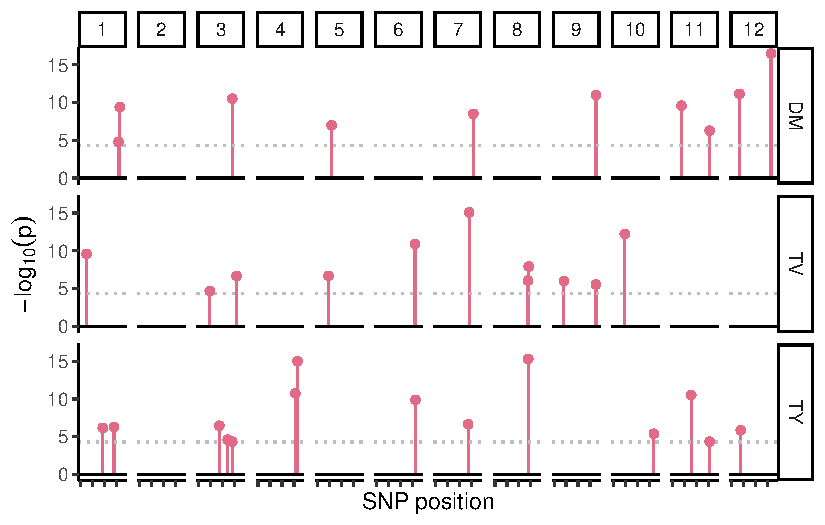
\includegraphics{figs_04/fig-lod-score-1.pdf}

}

\caption{\label{fig-lod-score}The physical positions and \(log_{10}\)
probabilities found for all 39 QTL across potato genome for dry matter
content (DM), tuber volume (TV), and total tuber yield (TY).}

\end{figure}
\section{Results}

\subsection{QTL Scan}\label{qtl-scan}

All scanning models converged successfully and picked up multiple QTL
for each phenotype (Table~\ref{tbl-summary}). The final QTL models
exhibited a better goodness of fit in contrast to the null model. This
was reflected both in the change of the AIC as well as reduction in
background genetic variance in each final model, though, this was trait
dependent. Between 53 and 56\% of the genetic variance was partitioned
away from the background genetic term between the null and final model
across traits. Among the traits tested, dry matter content appeared to
improve most through the incorporation of the 10 identified QTL
(Table~\ref{tbl-summary}).

In total, 35 QTL peaks were detected but given overlap between traits,
this comprised 33 unique QTL (Table~\ref{tbl-summary}). Total tuber
yield detected the largest number of QTLs (14 QTL) with tuber volume and
dry matter content detecting 11 and 10, respectively. The QTL variance
varied between 10 and 62\% of the total genetic variance among all
phenotypes but the median proportion of variance was highest in
drymatter content (36.0\%) followed by total tuber yield (30.1\%) and
average tuber volume (29\%) (Figure~\ref{fig-gen-size}). There were multiple QTL clusters detected for all three phenotypes comprising chromosome 1 for
dry matter content (chr01:83523334 and chr01:86604310), chromosome 8 in
tuber volume (chr08:46811267 and chr08:47889222), chromosome 4 in total
yield (chr04:60035708 and chr04:64373508).

\hypertarget{tbl-summary}{}
\begin{table}
\caption{\label{tbl-summary}Model parameters for the null and final QTL models for dry matter
content (DM), average tuber volume (TV) and total tuber yield (TY). The
Akaike Information Criterion (AIC), the change in AIC (\(\Delta AIC\)),
background genetic variance (\(\sigma^2_g\)), and per cent change in
background genetic variance (\(\Delta \% \)) for the initial
null and full QTL models. This is presented with the estimated global
mean of each trait and the total number of QTL incorporated into the
final model. }\tabularnewline

\centering
\begin{tabular}{ccccccccc}
\toprule
\multicolumn{1}{c}{ } & \multicolumn{3}{c}{AIC} & \multicolumn{3}{c}{$\sigma^2_g$} & \multicolumn{2}{c}{ } \\
\cmidrule(l{3pt}r{3pt}){2-4} \cmidrule(l{3pt}r{3pt}){5-7}
Phenotype & Null model & Final model & $\Delta$ & Null model & Final model & $\Delta\%$ & $\mu$ & Number of
QTL\\
\midrule
DM & 1690.0 & 1299.1 & 390.9 & 2.5 & 1.2 & 52.9 & 20.7 & 10\\
TV & 3650.0 & 3115.7 & 534.3 & 35.7 & 15.6 & 56.4 & 29.9 & 11\\
TY & 3394.1 & 2913.8 & 480.4 & 24.6 & 11.1 & 54.6 & 14.5 & 14\\
\bottomrule
\end{tabular}
\end{table}

\begin{figure}

{\centering 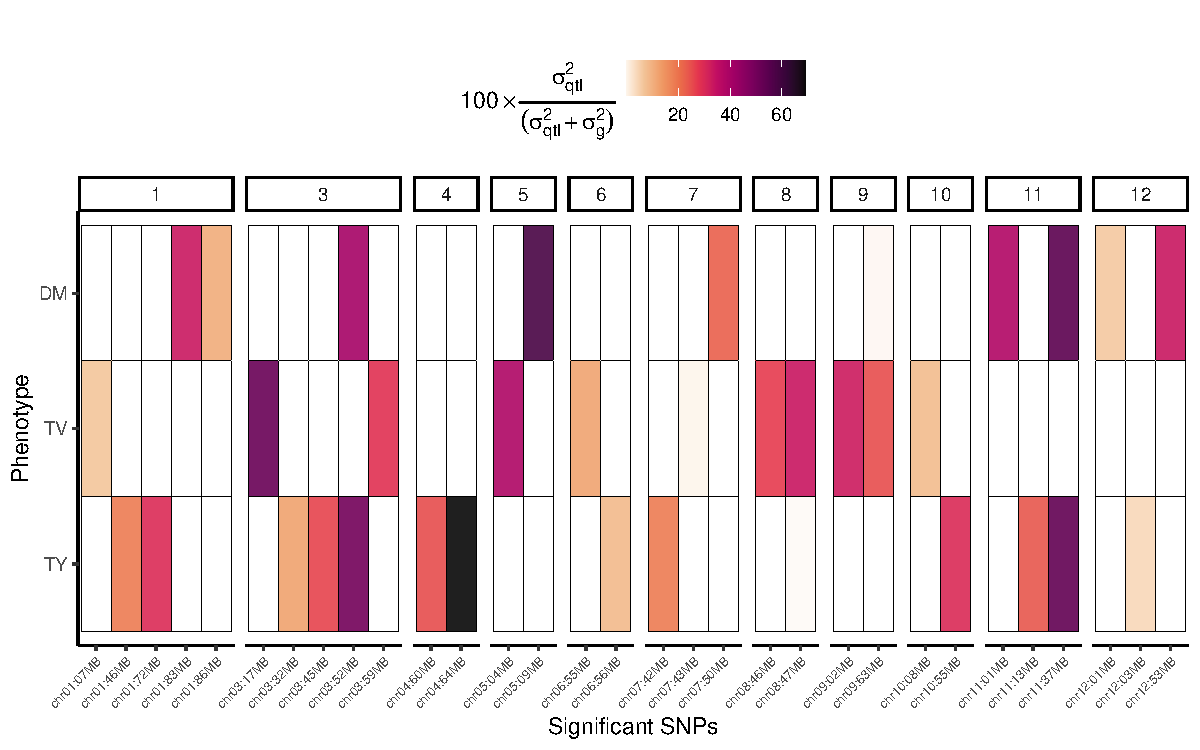
\includegraphics{figs_04/fig-gen-size-1.pdf}

}

\caption{\label{fig-gen-size}Proportion of captured genetic variance
from each QTL in the scanning model among all 35 identified QTL separated per chromosome in dry
matter content (DM), average tuber volume size (TV), and total tuber
yield (TY).}

\end{figure}

Examining all detected QTL, varying QTL effect size was observed with
respect to magnitude and direction (Figure~\ref{fig-snp-size}). The
largest QTL effects were observed in total tuber yield with effects as
large as 30\% of the mean. The QTL observed in dry matter content also
tended to be smaller in magnitude than those observed in tuber volume
and total tuber yield. Two correlated QTL were observed for dry matter
content and total tuber yield on chromosome 3 (chr03:52583805) and on
chromosome 11 (chr11:37618884) (Figure~\ref{fig-lod-score}). Both QTLs
had a relatively large QTL variance (Figure~\ref{fig-gen-size}) and were
negatively correlated between total tuber yield and dry matter content
(Figure~\ref{fig-snp-size}).

\begin{figure}

{\centering 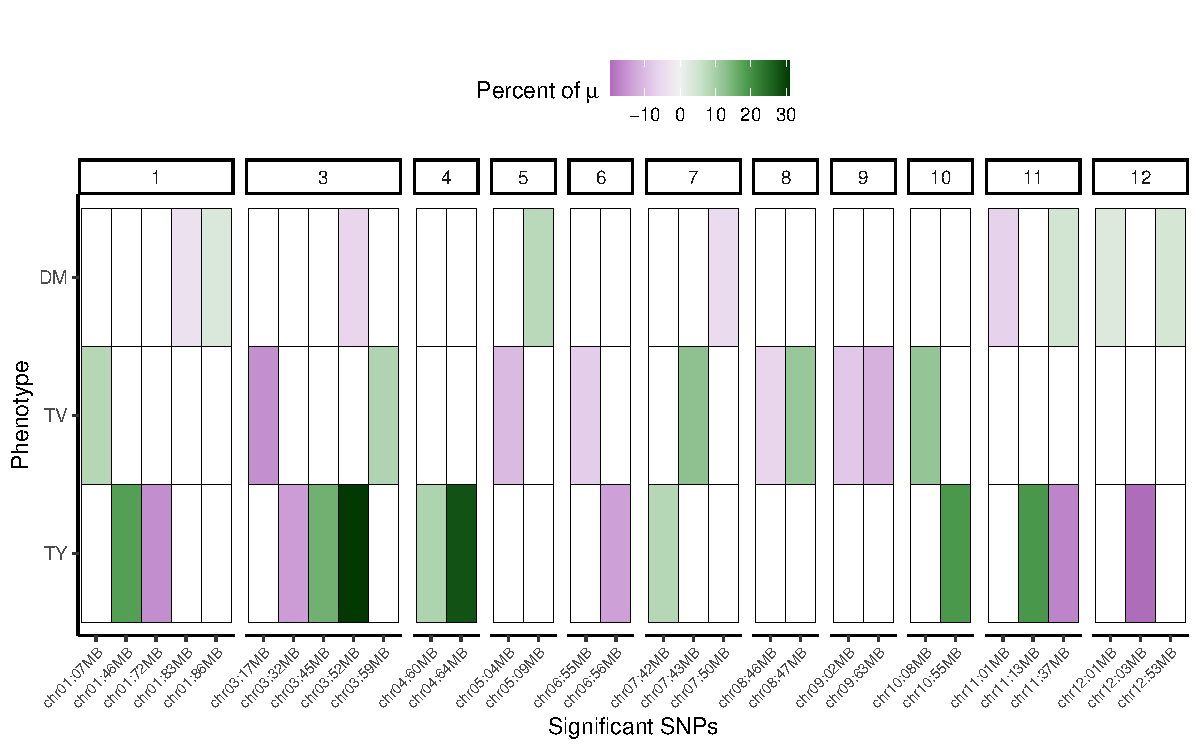
\includegraphics{figs_04/fig-snp-size-1.pdf}

}

\caption{\label{fig-snp-size}Marker effect size in \(\beta_{qtl}\) from
the final QTL model among all 35 identified QTL seperated per chromosome in dry matter content
(DM), average tuber volume size (TV), and total tuber yield (TY).}

\end{figure}

\begin{figure}

{\centering 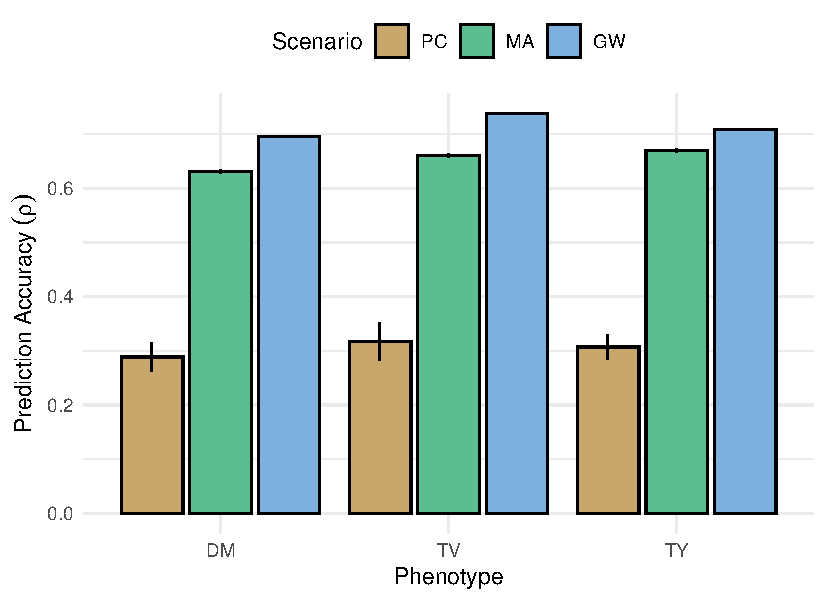
\includegraphics{figs_04/fig-pa-1.pdf}

}

\caption{\label{fig-pa}Prediction accuracy results from 5-fold cross
validation for qtl mapping (qtl), genome-wide regression (GW), and
marker-assisted selection with 12 random SNPs (PC). Error bars contain
one standard deviation around the average Pearson correlation
coefficient.}

\end{figure}

\hypertarget{genomic-prediction-models-1}{%
\subsection{Genomic Prediction
Models}\label{genomic-prediction-models-1}}

Turning to each predictive strategy, the \texttt{GW} scenario performed
consistently better than all other strategies and represented the maximum
prediction potential that could be attained (Figure~\ref{fig-pa}). It
also appears to closely mirror the phenotype heritabilities and
performance observed in previous studies (See \textcite{Adams2023}).
Conversely, the model used in \texttt{PC} were consistently the worst
performing with observed prediction accuracy's between 0.24 and 0.34 across
phenotypes. The \texttt{MA} models not only surpassed the negative
control (\texttt{PC}), but followed closely with the performance
observed in the \texttt{GW} model with \(\rho\)'s between 0.53 and 0.68
across traits. The \texttt{PC} strategy had the highest variability in
\(\rho\) during cross-validation due likely to the large probe sampling
variance. Examining these results relative to the \texttt{GW} scenario,
\texttt{MA} had a far larger relative efficiency for the three traits
targets (0.89 - 0.95) in contrast to \texttt{PC} (0.42 - 0.43)
(Table~\ref{tbl-re}). Looking to genotyping costs, the cost ratios varied very little between \texttt{MA} and \texttt{PC} strategies; both strategies were within two orders of magnitude cheaper than the \texttt{GW} genotyping strategy. All relative efficiencies were less than 1 but
when genotyping costs were considered, the \texttt{MA} was considerably
higher for all traits (1.41 - 1.48) indicative of higher selection
efficiencies per log cost. This was in contrast to the \texttt{PC}
scenario which had very low relative efficiency per log cost.
\section{Discussion}

An important exercise for any breeding program is the careful analysis
of goals for trait improvement in light of the genetic variation
present, the statistical architecture of the trait, and available
resources available to a program. Examining the
particular question of genotyping technology and selection methods, we
provide a template for evaluating the efficiency of breeding strategies.
In this paper, we were able to detect multiple QTL which captured a
large portion of the genetic variance in multiple tuber phenotypes. The
merit of these QTL were then tested through against a genome-wide
regression strategy and a random marker-based selection strategy as a
negative control. Selection responses were examined for all scenarios
with respect to unit gain and unit gain per unit cost. This represents
an invaluable procedure for assessing the benefits of two selection
methods in an operational breeding program.

\hypertarget{selecting-quantitative-traits}{%
\subsection{Selecting Quantitative
traits}\label{selecting-quantitative-traits}}

The first criteria for the success of quantitative trait selection is the
degree of genetic variability for the trait in question, in other words, 
the trait's heritability. Based upon the results of this study and previous
works \autocite{Adams2022} we know that all phenotypes studied here are highly
heritable and capable of genetic improvement. Based on prediction 
accuracy (Figure~\ref{fig-pa}) and consideration of
selection costs (Table~\ref{tbl-re}), we found credible evidence that
both MAS and genome-wide selection would be successful selection methods
for the traits studied here. Regarding genome-wide selection, this was in line with what other studies have observed for
these traits in potato \autocite{Adams2023,Wilson2021}. However, the
efficiency of the \texttt{MA} strategy for quantitative trait selection
needs further consideration. While MAS is an older technology and prone to lower selection accuracy's, it is still potentially an effective selection method
if sufficient genetic variation can be found. In our QTL mapping
procedure, over half the genetic variation was accounted for in the
final QTL model, and yet, the relative efficiency was as high as 0.95.
This could be a consequence of incorporating large effect QTL which
carry most of the relevant information for prediction. This was in
contrast to the \texttt{PC} control which, while having a similar number
of SNPs used for selection, offered little in way of selection
response. So given that there are still large effect QTL segregating
among candidates, the \texttt{MA} strategy is suitable in selection if
well designed markers are being used.

\hypertarget{tbl-re}{}
\begin{table}
\caption{\label{tbl-re}The relative efficiency (RE), genotyping cost ratio (CR) and relative efficiency per log cost
(\(\mathrm{RELC}\)) for the marker-assisted selection (MA) and the
single marker per chromosome strategies (PC) relative to the genome-wide
selection scenario (GW) for dry matter content (DM), average tuber
volume (TV), and total tuber yield (TY). }\tabularnewline

\centering
\begin{tabular}{ccccccc}
\toprule
\multicolumn{1}{c}{ } & \multicolumn{3}{c}{MA} & \multicolumn{3}{c}{PC} \\
\cmidrule(l{3pt}r{3pt}){2-4} \cmidrule(l{3pt}r{3pt}){5-7}
Phenotype & RE & CR & $\mathrm{RELC}$ & RE & CR & $\mathrm{RELC}$\\
\midrule
DM & 0.91 & 0.010 & 1.48 & 0.42 & 0.012 & 0.66\\
TV & 0.89 & 0.013 & 1.41 & 0.43 & 0.012 & 0.68\\
TY & 0.95 & 0.014 & 1.47 & 0.43 & 0.012 & 0.69\\
\bottomrule
\end{tabular}
\end{table}

\hypertarget{mas-versus-genome-wide-selection-costs-and-complexity}{%
\subsection{MAS versus genome-wide selection: Costs and
complexity}\label{mas-versus-genome-wide-selection-costs-and-complexity}}

When considering which of these strategies would be more appropriate for
employing in a hybrid potato breeding program, multiple questions need
to be considered. Most of these center around the maturity of the
breeding program and the priority of targets. Most crop breeding
programs are more conservative with genetic variation loss, and
therefore, would likely utilize a selection strategy which guarantees
the highest selection accuracy possible
\autocite{Swarup2021,Rasmusson1997}. In the context of these two tested
scenarios (\texttt{MA} and \texttt{GW}), this would lean towards the
genome-wide prediction approach. However, there are other programs that
could be less risk-adverse with regard to loss of genetic variation so
long as it allows for selection response (or unit selection response per
unit cost) to be maximized by some other means. We observed that when
considering genotyping costs, the \texttt{MA} strategy was more
efficient per log cost for all three trait targets (Table~\ref{tbl-re}).
When a cost penalty is introduced, any affordable technology that
borders with the performance of genome-wide regression becomes
immediately interesting for adoption. So for breeding programs which
value greater or more cost-efficient short-term gains, a marker-assisted
selection approach is worth consideration for quantitative trait
selection.

\hypertarget{operational-considerations}{%
\subsection{Operational
considerations}\label{operational-considerations}}

These scenarios are presented as is with no formal consideration of
other operational questions which could be relevant for their effective
adoption. For example, we used a population where QTLs could be
identified, however, this is of course not guaranteed. The success of
QTL identification in a breeding program is dependent on many
interrelated questions: population mapping or family mapping
\autocite{Wurschum2012}, having dedicated mapping populations or using
extant material, and the number of individuals used
\autocite{Lande1990}. Even after QTL identification, there are common
pitfalls in maintaining a marker in a MAS program such as recombination
between the QTL and marker, ensuring universal probe annealing across
relevant genetic backgrounds, and maintaining these targets alongside
other important genes necessary for a candidate's portfolio. Genome-wide
prediction methods in this regard, are more straightforward, as model
training, testing, validation, and retraining are regular procedures as
breeding populations develop over time. However, an unappreciated
logistical challenge with such predictive workflows is proper investment
in data management and well engineered data pipelines as the size of
datasets accumulate each year. The creation and maintenance of such
digital infrastructure for genomic workloads requires expertise outside
of the genetical and statistical domain and could be a liability if not
sufficiently planned accordingly \autocite{ODriscoll2013,Mulder2017}.

\section{Conclusions} % (fold)

Complex traits in field crops include some of the most economically
valuable targets for trait improvement such as biomass partitioning, abiotic
stress resistance, and crop yield. Therefore, identifying schema which
maximize the rate of genetic progress in candidate selection is an
indispensable activity for breeding programs. Here we focused our attention 
on three important yield phenotypes in potato and found that MAS could serve
as an affordable selection methodology in the place of genome-wide predictive
methods. Such a low-cost technology lends itself to allocation bottlenecks common
to breeding programs where the number of candidates are large, a scenario common to 
multiple stages of a hybrid breeding program. Tools like MAS are thus still a valuable part of the
 breeders toolbox for genetic improvement in hybrid potato.
